\ifx\allfiles\undefined
\documentclass[12pt, a4paper, oneside, UTF8]{ctexbook}
\usepackage{amsmath}   % 数学公式
\usepackage[dvipsnames]{xcolor}
\usepackage{amsthm}    % 定理环境
\usepackage{amssymb}   % 更多公式符号
\usepackage{graphicx}  % 插图
\usepackage{mathrsfs}  % 数学字体
\usepackage{enumitem}  % 列表
\usepackage{geometry}  % 页面调整
\usepackage{unicode-math}
\usepackage{extarrows}
\usepackage{subfigure}
\usepackage{extarrows}
\usepackage{footnote}
\usepackage{svg}
\usepackage[colorlinks,linkcolor=black]{hyperref}
\usepackage{supertabular}
\usepackage{tcolorbox}
\usepackage{ulem}
\usepackage{framed}
\usepackage{float}
\usepackage{microtype}
\newcommand{\arccot}{\mathrm{arccot}\,}
\tcbuselibrary{breakable}
\tcbuselibrary{most}
\newcounter{problemname}
\newenvironment{solution}{\par\noindent\textbf{解答. }}{\par}
\newenvironment{note}{\par\noindent\textbf{题目\arabic{problemname}的注记. }}{\par}
\definecolor{shadecolor}{RGB}{241, 241, 255}
\newenvironment{problem}{\begin{shaded}\stepcounter{problemname}\par\noindent\textbf{题目\arabic{problemname}. }}{\end{shaded}\par}

\graphicspath{ {figure/},{../figure/}, {config/}, {../config/} }  % 配置图形文件检索目录
\linespread{1.2} % 行高

% 页码设置
\geometry{top=25.4mm,bottom=25.4mm,left=20mm,right=20mm,headheight=2.17cm,headsep=4mm,footskip=12mm}

% 设置列表环境的上下间距
\setenumerate[1]{itemsep=5pt,partopsep=0pt,parsep=\parskip,topsep=5pt}
\setitemize[1]{itemsep=5pt,partopsep=0pt,parsep=\parskip,topsep=5pt}
\setdescription{itemsep=5pt,partopsep=0pt,parsep=\parskip,topsep=5pt}

% 定理环境
% ########## 定理环境 start ####################################

% #### 将 config.tex 中的定理环境的对应部分替换为如下内容
% 定义单独编号,其他四个共用一个编号计数 这里只列举了五种,其他可类似定义(未定义的使用原来的也可)
\newtcbtheorem[auto counter, number within=section, list type=subsubsection, list inside=toc]{defn}{定义}
{
    colback=green!5,colframe=green!35!black,fonttitle=\bfseries, title={Comment \thetcbcounter}, list entry={Comment \thetcbcounter\quad}, %标题
    breakable, %支持跨页
    before upper={\parindent10pt\noindent},  % 支持缩进。\noindent:首行不缩进
    % left = 2mm, %文字离线框左边的边距
    % right = 1mm,%同上
    % top = 1mm,%同上
    % bottom = 1mm,%同上
    % arc is angular = 1mm, % 棱角线框
    % sharp corners, % 直角线框
    % enhanced,frame hidden, % 隐藏线框
    % enhanced, drop fuzzy shadow,  % 显示阴影
}
{def}

\newtcbtheorem[auto counter, number within=section, list type=subsubsection, list inside=toc]{lemma}{引理}
{
    colback=SeaGreen!10!CornflowerBlue!10,colframe=RoyalPurple!55!Aquamarine!100!,fonttitle=\bfseries, title={Comment \thetcbcounter}, list entry={Comment \thetcbcounter\quad}, %标题
    breakable, %支持跨页
    before upper={\parindent10pt\noindent},  % 支持缩进。\noindent:首行不缩进
    % left = 2mm, %文字离线框左边的边距
    % right = 1mm,%同上
    % top = 1mm,%同上
    % bottom = 1mm,%同上
    % arc is angular = 1mm, % 棱角线框
    % sharp corners, % 直角线框
    % enhanced,frame hidden, % 隐藏线框
    % enhanced, drop fuzzy shadow,  % 显示阴影
}
{lem}


\newtcbtheorem[auto counter, number within=section, list type=subsubsection, list inside=toc]{them}{定理}
{
    colback=Salmon!20, colframe=Salmon!90!Black,fonttitle=\bfseries, title={Comment \thetcbcounter}, list entry={Comment \thetcbcounter\quad}, %标题
    breakable, %支持跨页
    before upper={\parindent10pt\noindent},  % 支持缩进。\noindent:首行不缩进
    % left = 2mm, %文字离线框左边的边距
    % right = 1mm,%同上
    % top = 1mm,%同上
    % bottom = 1mm,%同上
    % arc is angular = 1mm, % 棱角线框
    % sharp corners, % 直角线框
    % enhanced,frame hidden, % 隐藏线框
    % enhanced, drop fuzzy shadow,  % 显示阴影
}
{them}
\newtcbtheorem[auto counter, number within=section, list type=subsubsection, list inside=toc]{criterion}{注}
{
    colback=CornflowerBlue!10,colframe=RoyalPurple!55!Aquamarine!100!,fonttitle=\bfseries, title={Comment \thetcbcounter}, list entry={Comment \thetcbcounter\quad}, %标题
    breakable, %支持跨页
    before upper={\parindent10pt\noindent},  % 支持缩进。\noindent:首行不缩进
    % left = 2mm, %文字离线框左边的边距
    % right = 1mm,%同上
    % top = 1mm,%同上
    % bottom = 1mm,%同上
    % arc is angular = 1mm, % 棱角线框
    % sharp corners, % 直角线框
    % enhanced,frame hidden, % 隐藏线框
    % enhanced, drop fuzzy shadow,  % 显示阴影
}
{cri}

\newtcbtheorem[auto counter, number within=section, list type=subsubsection, list inside=toc]{corollary}{推论}
{
    colback=Emerald!10,colframe=cyan!40!black,fonttitle=\bfseries, title={Comment \thetcbcounter}, list entry={Comment \thetcbcounter\quad}, %标题
    breakable, %支持跨页
    before upper={\parindent10pt\noindent},  % 支持缩进。\noindent:首行不缩进
    % left = 2mm, %文字离线框左边的边距
    % right = 1mm,%同上
    % top = 1mm,%同上
    % bottom = 1mm,%同上
    % arc is angular = 1mm, % 棱角线框
    % sharp corners, % 直角线框
    % enhanced,frame hidden, % 隐藏线框
    % enhanced, drop fuzzy shadow,  % 显示阴影
}
{cor}
% colback=red!5,colframe=red!75!black

% ######### 定理环境 end  #####################################

% ↓↓↓↓↓↓↓↓↓↓↓↓↓↓↓↓↓ 以下是自定义的命令  ↓↓↓↓↓↓↓↓↓↓↓↓↓↓↓↓

% 用于调整表格的高度  使用 \hline\xrowht{25pt}
\newcommand{\xrowht}[2][0]{\addstackgap[.5\dimexpr#2\relax]{\vphantom{#1}}}

% 表格环境内长内容换行  
\newcommand{\tabincell}[2]{\begin{tabular}{@{}#1@{}}#2\end{tabular}}

% 使用\linespread{1.5} 之后 cases 环境的行高也会改变,重新定义一个 ca 环境可以自动控制 cases 环境行高
\newenvironment{ca}[1][1]{\linespread{#1} \selectfont \begin{cases}}{\end{cases}}
% 和上面一样
\newenvironment{vx}[1][1]{\linespread{#1} \selectfont \begin{vmatrix}}{\end{vmatrix}}

\def\d{\textup{d}} % 直立体 d 用于微分符号 dx
\def\R{\mathbb{R}} % 实数域
\newcommand{\bs}[1]{\boldsymbol{#1}}    % 加粗,常用于向量
\newcommand{\ora}[1]{\overrightarrow{#1}} % 向量

% 数学 平行 符号
\newcommand{\pll}{\kern 0.5em/\kern -0.8em /\kern 0.5em}

% 用于空行\myspace{1} 表示空一行 填 2 表示空两行  
\newcommand{\myspace}[1]{\par\vspace{#1\baselineskip}}

\begin{document}
% \title{{\Huge{\textbf{高等数学笔记}}}}
\author{作者:于家崇}
\date{\today}
\maketitle                   % 在单独的标题页上生成一个标题

\thispagestyle{empty}        % 前言页面不使用页码
\begin{center}
	\Huge\textbf{前言}
\end{center}

If a job is worth doing,it's worth doing well
\begin{flushright}
	\begin{tabular}{c}
		\today \\ 如果一件事值得去做,那就值得去做好
	\end{tabular}
\end{flushright}

\newpage                      % 新的一页
\pagestyle{plain}             % 设置页眉和页脚的排版方式(plain:页眉是空的,页脚只包含一个居中的页码)
\setcounter{page}{1}          % 重新定义页码从第一页开始
\pagenumbering{Roman}         % 使用大写的罗马数字作为页码
\tableofcontents              % 生成目录

\newpage                      % 以下是正文
\pagestyle{plain}
\setcounter{page}{1}          % 使用阿拉伯数字作为页码
\pagenumbering{arabic}
% \setcounter{chapter}{-1}    % 设置 -1 可作为第零章绪论从第零章开始 
\else
\fi
%  ############################ 正文部分
\chapter{连续}

\section{函数的连续性}
连续函数是一条连续而不间断的曲线,以下为函数连续的两个定义
\begin{defn}{}{}
    设函数$y=f(x)$在点$x_0$的某一邻域内有定义,如果
    $$
        \lim_{\Delta x\to0}\Delta y=\lim_{\Delta x\to0}\big[f\big(x_{0}+\Delta x\big)-f\big(x_{0}\big)\big]=0
    $$
    那就称为函数$y=f(x)$在点$x_0$连续.
\end{defn}
\begin{defn}{}{}
    设函数$y=f(x)$在点$x_0$的某一邻域有定义,如果
    $$
        \underset{x\to x_0}{\operatorname*{lim}}f(x)=f(x_0)
    $$
    那么就称函数$f(x)$在点$x_0$连续
    其$\varepsilon - \delta $语言表达如下:\\
    $f(x)\text{ 在点 }x_0\text{连续}\Leftrightarrow\forall\boldsymbol{\varepsilon}>0,\exists\delta>0,\text{当}|x-x_0|<\delta\text{ 时 },\text{有}|f(x)-f(x_0)|<\varepsilon $
\end{defn}
\subsection{反函数与复合函数的连续性}
\begin{defn}{}{}
    如果函数$y=f(x)$在区间$I_x$上单调增加(或单调减少)且连续那么它的反函数 $x=f^{-1}(y)$也在对应的区间$I_{y}=\{\text{ y | y = }f(x),x\in I_{x}\}$上单调增加(或单调减少)且连续
\end{defn}
\begin{defn}{}{}
    设函数$y=f\Big[g(x)\Big]$由函数$u=g(x)$与函数 $y=f(u)$复合而成$\stackrel{\circ}{U}(x_0)\subset D_{f,g}$.若$\lim_{x\to x_0}g(x)=u_0$,而函数 $y=f(u)$在$u=u_0$连续,则
    $$\operatorname*{lim}_{x\to x_0}f\Big[g(x)\Big]=\operatorname*{lim}_{u\to u_0}f(u)=f(u_0)$$
\end{defn}
\subsection{初等函数的连续性}
\begin{defn}{}{}
    \begin{itemize}
        \item 基本初等函数在其定义域内都连续
        \item 初等函数在其定义区间内都连续
    \end{itemize}
\end{defn}
\subsection{闭区间上连续函数的性质}

\subsubsection{有界性与最大值最小值定理}
\begin{defn}{最值定理}{}
    在闭区间上连续的函数在该区间上有界且一定能取得它的最大值和最 小值
\end{defn}
% 3.1.1
\subsubsection{零点定理与介值定理}
% 3.1.2
\begin{defn}{零点定理}{}
    设函数$f(x)$在闭区间$\left[\begin{array}{c}a,b\end{array}\right]$上连续,且$f(\begin{array}{c}a\end{array})$与$f(\begin{array}{c}b\end{array})$ 异号(即$f(\begin{array}{c}a\end{array})\cdot f(\textit{ b )<}0)$,则在开区间$(a,b)$内至少有一点$\xi$,使$f(\xi)=0$.
\end{defn}
\begin{defn}{介值定理}{}
    设函数$f(x)$在闭区间$[a,b]$上连续,且在这区间的端点取不同的函数值,
    $$
        f(a)=A \text{及} f(b)=B
    $$
    则对于$A$与$B$之间的任意一个数$C$,在开区间$(a,b)$内至少存在一点$\xi$,使得
    $$
        f(\xi) =C (a< \xi <b)
    $$
\end{defn}
该定理的几何意义是:连续曲线弧$y=f(x)$与水平直线$y=C$至少存在相交于一点.
\section{函数的间断点}
\subsection{间断点的相关概念}
\begin{itemize}
    \item 可去间断点:若$\lim_{x\to x_0}f(x)=A\neq f(x_0)(f(x_0)$甚至可以无定义),则这类间断点称为可去间断点
          \begin{figure}[H]
              \centering 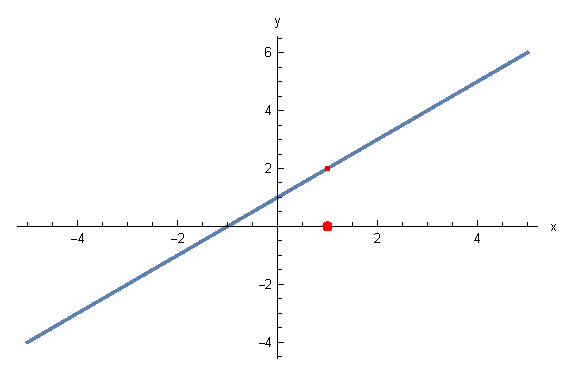
\includegraphics[width=
                  0.4 \linewidth]{3.2.1.eps} \caption{可去间断点函数图像}
          \end{figure}
    \item 跳跃间断点:若$\lim_{x\to x_0^-}f(x)$与$\lim_{x\to x_0^+}f(x)$都存在,但$\lim_{x\to x_0^+}f(x)\neq\lim_{x\to x_0^-}f(x)$,则这类间断点称为跳跃间断点
          \begin{figure}[H]
              \centering 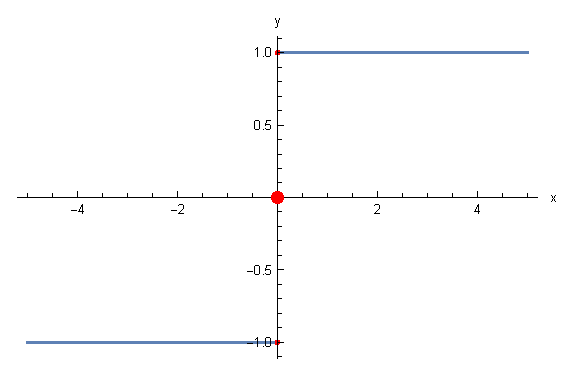
\includegraphics[width=
                  0.4 \linewidth]{3.2.2.eps} \caption{跳跃间断点函数图像}
          \end{figure}
    \item 无穷间断点:若$\lim_{x\to x_0}f(x)=\infty$,则这类间断点称为无穷间断点,如$y=\tan x$
          \begin{figure}[H]
              \centering 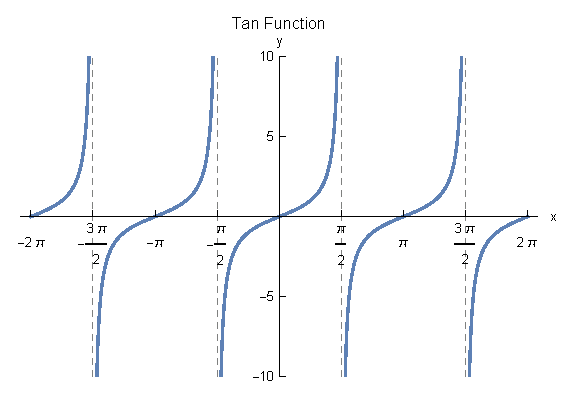
\includegraphics[width=
                  0.4 \linewidth]{1.3.6.eps} \caption{无穷间断点函数tan图像}
          \end{figure}
    \item 振荡间断点:若$\lim_{x\to x_0}f(x)$振荡不存在,则这类间断点称为振荡间断点
          \begin{figure}[H]
              \centering 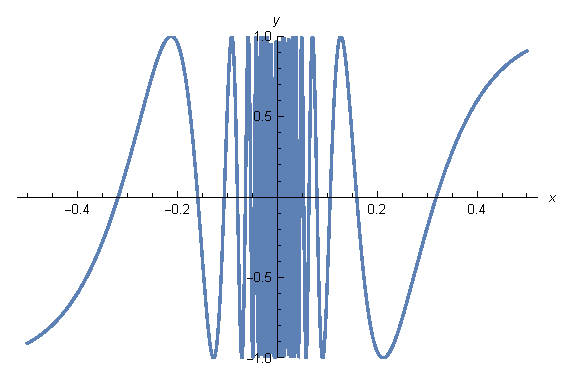
\includegraphics[width=
                  0.4 \linewidth]{3.2.3.eps} \caption{振荡间断点函数$\sin \frac{1}{x}$图像}
          \end{figure}
\end{itemize}
\subsection{间断点的分类}
通过求函数在该点的左右极限来判断
\begin{itemize}
    \item 第一类间断点:$\lim _ { x \rightarrow x _ { 0 } ^{-}} f ( x )$​ 和$\lim _ { x \rightarrow x _ { 0 }^ {+}} f ( x )$​ 均存在
          \begin{itemize}
              \item 可去:$\lim _ { x \rightarrow x_0 ^ { - } } f ( x ) = \lim _ { x \rightarrow x_0^{+} } f  ( x ) \neq f(x_0)$
              \item 跳跃:$\lim _ { x \rightarrow x_0^{-} } f ( x ) \not= \lim _ { x \rightarrow x_0^{+} } f ( x )$
          \end{itemize}
    \item 第二类间断点:除第一类以外的间断点$\implies \lim _ { x \rightarrow x _ { 0 } ^{-}} f ( x )$和$\lim _ { x \rightarrow x _ { 0 }^ {+}} f ( x )$​ 均至少一个不存在
\end{itemize}
%  ############################ 正文部分
\ifx\allfiles\undefined
\end{document}
\fi
